\documentclass[dvipsnames,border=3pt]{standalone}
\usepackage{tikz}
\usetikzlibrary{arrows}
\usetikzlibrary{shapes}
\usepackage{enumitem}
\usepackage{bm}
\usepackage{mathdots}
\usepackage{amsmath}
\usetikzlibrary{shadings}
\usetikzlibrary{decorations.pathreplacing}
\usepackage{helvet}
\usetikzlibrary{arrows.meta}
\usepackage{graphicx}
\usepackage{pgfplots}
\usepackage{pgfplotstable}
\usepackage{filecontents}
\usetikzlibrary{plotmarks}
\pgfplotsset{compat=newest}

\renewcommand{\familydefault}{\sfdefault}

\definecolor{mylightgray}{cmyk}{0,0,0,0.1}
\usetikzlibrary{arrows,decorations.pathmorphing,backgrounds,fit,positioning,shapes.symbols,chains}

\begin{document}

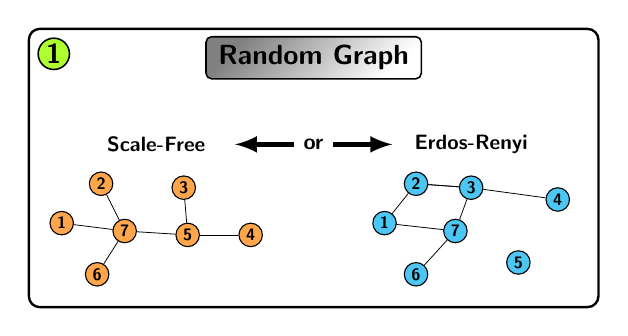
\begin{tikzpicture}
    % trim=left botm right top
    
%%%%%%%%%%%%%%%%%%%%%%%%%%%%%%%%%%%%%%%%%%%%%%%%%%%%%%%%%%%%%%%%%%%%%%%%%%%%%%%%%%%%%%%%%%%%%%%%%%
%%%%%%%%%%%%%%%%%%%%%%%%%%%%%%%%%%%%%%%%%%% box 1 %%%%%%%%%%%%%%%%%%%%%%%%%%%%%%%%%%%%%%%%%%%%%%%%
%%%%%%%%%%%%%%%%%%%%%%%%%%%%%%%%%%%%%%%%%%%%%%%%%%%%%%%%%%%%%%%%%%%%%%%%%%%%%%%%%%%%%%%%%%%%%%%%%%

\node[draw, rounded corners=4, line width=0.3mm, text width=7cm, text height=3.3cm] at (0,-1.1) {};
\node[circle,draw,line width=0.2mm,xscale=1.2,yscale=1.2,fill=GreenYellow] at (-3.3,0.35) {};
\node at (-3.3,0.35) {\textbf{1}};

%%%%%%%%%%%%%%%%%%%%%%%%%%%%%%%%%%%%%%%%%%%%%%%%%%%%%%%%%%%%%%%%%%%%%%%%%%%%%%%%%%%%%%%%%%%%%%%%%%
%%%%%%%%%%%%%%%%%%%%%%%%%%%%%%%%%%%%%%%%%%% box 1 %%%%%%%%%%%%%%%%%%%%%%%%%%%%%%%%%%%%%%%%%%%%%%%%
%%%%%%%%%%%%%%%%%%%%%%%%%%%%%%%%%%%%%%%%%%%%%%%%%%%%%%%%%%%%%%%%%%%%%%%%%%%%%%%%%%%%%%%%%%%%%%%%%%

\node[draw,rounded corners=2,line width=0.2mm,fill=gray!50,text height=0.3cm, text width=2.5cm,shading angle=45] at (0,0.3) {}; % random graph
\node at (0,0.3) {\textbf{Random Graph}};

%\node[draw,line width=0.2mm,rounded corners=2,text height=0.2cm,text width=1.4cm] at (-2,-1) {};
\node[xscale=0.75,yscale=0.75] at (-2,-0.8) {\textbf{Scale-Free}}; % scale-free

%\node[draw,line width=0.2mm,rounded corners=2,text height=0.2cm,text width=1.4cm] at (2,-1) {};
\node[xscale=0.75,yscale=0.75] at (2,-0.8) {\textbf{Erdos-Renyi}}; % erdos-renyi

%%%%%%%%%%%%%%%%%%%%%%%%%%%%%%%%%%%%%%%%%%%%%%%%%%%%%%%%%%%%%%%%%%%%%%%%%%%%%%%%%%%%%%%%%%%%%%%%%%
%%%%%%%%%%%%%%%%%%%%%%%%%%%%%%%%%%%%% scale-free graph %%%%%%%%%%%%%%%%%%%%%%%%%%%%%%%%%%%%%%%%%%%
%%%%%%%%%%%%%%%%%%%%%%%%%%%%%%%%%%%%%%%%%%%%%%%%%%%%%%%%%%%%%%%%%%%%%%%%%%%%%%%%%%%%%%%%%%%%%%%%%%

\node[circle,draw,xscale=0.9,yscale=0.9, fill=orange!70!] at (-3.2,-1.8) (1) {};
\node[xscale=0.6,yscale=0.6] at (-3.2,-1.8) {\textbf{1}}; % node 1

\node[circle,draw,xscale=0.9,yscale=0.9, fill=orange!70!] at (-2.7,-1.3) (2) {};
\node[xscale=0.6,yscale=0.6] at (-2.7,-1.3) {\textbf{2}}; % node 2

\node[circle,draw,xscale=0.9,yscale=0.9, fill=orange!70!] at (-2.4,-1.9) (7) {};
\node[xscale=0.6,yscale=0.6] at (-2.4,-1.9) {\textbf{7}}; % node 7

\node[circle,draw,xscale=0.9,yscale=0.9, fill=orange!70!] at (-1.6,-1.95) (5) {};
\node[xscale=0.6,yscale=0.6] at (-1.6,-1.95) {\textbf{5}}; % node 5

\node[circle,draw,xscale=0.9,yscale=0.9, fill=orange!70!] at (-0.8,-1.95) (4) {};
\node[xscale=0.6,yscale=0.6] at (-0.8,-1.95) {\textbf{4}}; % node 4

\node[circle,draw,xscale=0.9,yscale=0.9, fill=orange!70!] at (-1.65,-1.35) (3) {};
\node[xscale=0.6,yscale=0.6] at (-1.65,-1.35) {\textbf{3}}; % node 3

\node[circle,draw,xscale=0.9,yscale=0.9, fill=orange!70!] at (-2.75,-2.45) (6) {};
\node[xscale=0.6,yscale=0.6] at (-2.75,-2.45) {\textbf{6}}; % node 6

\draw[line width=0.1mm] (1) -- (7);
\draw[line width=0.1mm] (7) -- (2);
\draw[line width=0.1mm] (6) -- (7);
\draw[line width=0.1mm] (5) -- (7);
\draw[line width=0.1mm] (5) -- (3);
\draw[line width=0.1mm] (5) -- (4);

%%%%%%%%%%%%%%%%%%%%%%%%%%%%%%%%%%%%%%%%%%%%%%%%%%%%%%%%%%%%%%%%%%%%%%%%%%%%%%%%%%%%%%%%%%%%%%%%%%
%%%%%%%%%%%%%%%%%%%%%%%%%%%%%%%%%%%%% scale-free graph %%%%%%%%%%%%%%%%%%%%%%%%%%%%%%%%%%%%%%%%%%%
%%%%%%%%%%%%%%%%%%%%%%%%%%%%%%%%%%%%%%%%%%%%%%%%%%%%%%%%%%%%%%%%%%%%%%%%%%%%%%%%%%%%%%%%%%%%%%%%%%

\draw[-latex, line width=0.6mm] (-0.25,-0.8) -- (-1,-0.8);
\node[xscale=0.8,yscale=0.8] at (0,-0.8) {\textbf{or}};
\draw[-latex, line width=0.6mm] (0.25,-0.8) -- (1,-0.8);

%%%%%%%%%%%%%%%%%%%%%%%%%%%%%%%%%%%%%%%%%%%%%%%%%%%%%%%%%%%%%%%%%%%%%%%%%%%%%%%%%%%%%%%%%%%%%%%%%%
%%%%%%%%%%%%%%%%%%%%%%%%%%%%%%%%%%%%% erdos-renyi graph %%%%%%%%%%%%%%%%%%%%%%%%%%%%%%%%%%%%%%%%%%
%%%%%%%%%%%%%%%%%%%%%%%%%%%%%%%%%%%%%%%%%%%%%%%%%%%%%%%%%%%%%%%%%%%%%%%%%%%%%%%%%%%%%%%%%%%%%%%%%%

\node[circle,draw,xscale=0.9,yscale=0.9, fill=cyan!70!] at (0.9,-1.8) (1) {};
\node[xscale=0.6,yscale=0.6] at (0.9,-1.8) {\textbf{1}}; % node 1

\node[circle,draw,xscale=0.9,yscale=0.9, fill=cyan!70!] at (1.3,-1.3) (2) {};
\node[xscale=0.6,yscale=0.6] at (1.3,-1.3) {\textbf{2}}; % node 2

\node[circle,draw,xscale=0.9,yscale=0.9, fill=cyan!70!] at (1.8,-1.9) (7) {};
\node[xscale=0.6,yscale=0.6] at (1.8,-1.9) {\textbf{7}}; % node 7

\node[circle,draw,xscale=0.9,yscale=0.9, fill=cyan!70!] at (2.6,-2.3) (5) {};
\node[xscale=0.6,yscale=0.6] at (2.6,-2.3) {\textbf{5}}; % node 5

\node[circle,draw,xscale=0.9,yscale=0.9, fill=cyan!70!] at (3.1,-1.5) (4) {};
\node[xscale=0.6,yscale=0.6] at (3.1,-1.5) {\textbf{4}}; % node 4

\node[circle,draw,xscale=0.9,yscale=0.9, fill=cyan!70!] at (2,-1.35) (3) {};
\node[xscale=0.6,yscale=0.6] at (2,-1.35) {\textbf{3}}; % node 3

\node[circle,draw,xscale=0.9,yscale=0.9, fill=cyan!70!] at (1.3,-2.45) (6) {};
\node[xscale=0.6,yscale=0.6] at (1.3,-2.45) {\textbf{6}}; % node 6

\draw[line width=0.1mm] (1) -- (7);
\draw[line width=0.1mm] (2) -- (3);
\draw[line width=0.1mm] (6) -- (7);
\draw[line width=0.1mm] (3) -- (7);
\draw[line width=0.1mm] (2) -- (3);
\draw[line width=0.1mm] (3) -- (4);
\draw[line width=0.1mm] (1) -- (2);

%%%%%%%%%%%%%%%%%%%%%%%%%%%%%%%%%%%%%%%%%%%%%%%%%%%%%%%%%%%%%%%%%%%%%%%%%%%%%%%%%%%%%%%%%%%%%%%%%%
%%%%%%%%%%%%%%%%%%%%%%%%%%%%%%%%%%%%% erdos-renyi graph %%%%%%%%%%%%%%%%%%%%%%%%%%%%%%%%%%%%%%%%%%
%%%%%%%%%%%%%%%%%%%%%%%%%%%%%%%%%%%%%%%%%%%%%%%%%%%%%%%%%%%%%%%%%%%%%%%%%%%%%%%%%%%%%%%%%%%%%%%%%%

    
\end{tikzpicture}
    
\end{document}